%%%%%%%%%%%%%%%%%%%%%%%%%%%%%%%%%%%%%%%%%%%%%%%%%%%%%
%                                                   %
%     Penn State Colloquium Poster Template         %
%                                                   %
% Uses Penn State Colloquium class, with options:   %
%                                                   %
% Orientation:                                      %
%     portrait (default), landscape                 %
%                                                   %
% Paper size:                                       %
%     a4paper (default), a0paper, a1paper, a2paper, %
%     a3paper, a5paper, a6paper                     %
%%%%%%%%%%%%%%%%%%%%%%%%%%%%%%%%%%%%%%%%%%%%%%%%%%%%%
\documentclass{../psuposter}
\renewcommand{\templateimagepath}{../} 


%%%%%%%%%%%%%%%%%%%%%%%%%%%%%%%%%%%%%%%%%%%%%%%%%%%%%
%               Package Dependencies                %
%%%%%%%%%%%%%%%%%%%%%%%%%%%%%%%%%%%%%%%%%%%%%%%%%%%%%
\usepackage{natbib}
\usepackage{lipsum}                                % Dummy text
\usepackage[figwidth = 0.98\linewidth]{todonotes}  % Dummy image (and more!)
\usepackage[absolute, overlay]{textpos}            % Figure placement
\usepackage{braket}
\setlength{\TPHorizModule}{\paperwidth}
\setlength{\TPVertModule}{\paperheight}
\setcitestyle{numbers,square}


%%%%%%%%%%%%%%%%%%%%%%%%%%%%%%%%%%%%%%%%%%%%%%%%%%%%%
%                 AUTHOR AND TITLE                  %
%%%%%%%%%%%%%%%%%%%%%%%%%%%%%%%%%%%%%%%%%%%%%%%%%%%%%
\title{Comparative neurobiology of vocal communication}
\author{Michael Long}
\institute{School of Medicine, New York University}


%%%%%%%%%%%%%%%%%%%%%%%%%%%%%%%%%%%%%%%%%%%%%%%%%%%%%
%                  BEGIN DOCUMENT                   %
%%%%%%%%%%%%%%%%%%%%%%%%%%%%%%%%%%%%%%%%%%%%%%%%%%%%%
\begin{document}
\begin{frame}
\begin{columns}[t, totalwidth=\textwidth]
\begin{column}{0.45\textwidth - 1cm}


%%%%%%%%%%%%%%%%%%%%%%%%%%%%%%%%%%%%%%%%%%%%%%%%%%%%%
%                 BLOCK: BIOGRAPHY                  %
%%%%%%%%%%%%%%%%%%%%%%%%%%%%%%%%%%%%%%%%%%%%%%%%%%%%%
    \begin{block}{Speaker Biographic Summary}
    	\begin{center}
    		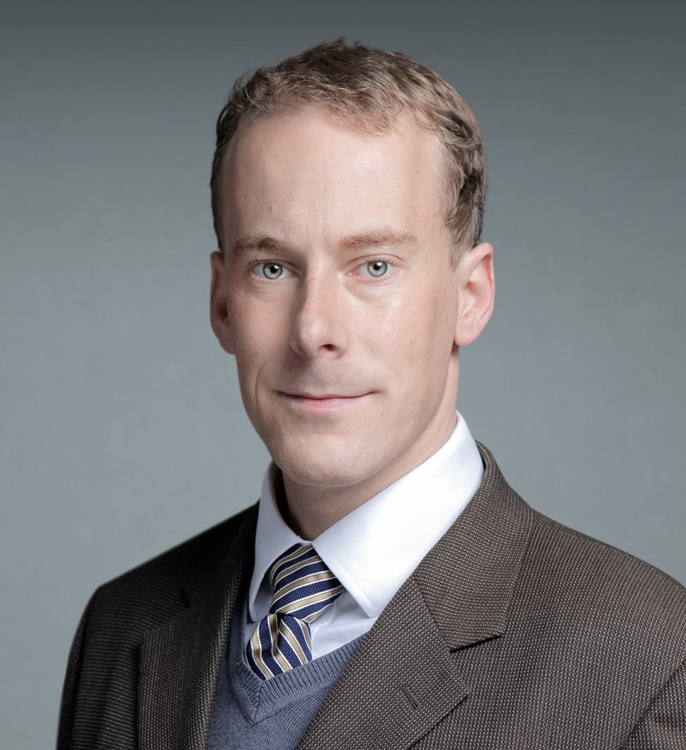
\includegraphics[width=0.68\textwidth]{images/long}
    	\end{center}
    	\href{https://med.nyu.edu/faculty/michael-a-long}{Dr. Michael Long} is
    	an Associate Professor in the Department of Otolaryngology-Head and Neck Surgery at New York University, and the Thomas and Suzanne Murphy Associate Professor of Neuroscience and Physiology in the Department of Neuroscience and Physiology at New York University. He is also an  Executive Director at New York University Langone Health, and is affiliated with the Neuroscience Institute. He trained with Dr. Barry Connors at Brown University, where he completed his Ph.D., and studied with Dr. Michale Fee at MIT. Dr. Long's work analyses the neural circuits that underlie complex behavior. 
    \end{block}


%%%%%%%%%%%%%%%%%%%%%%%%%%%%%%%%%%%%%%%%%%%%%%%%%%%%%
%            BLOCK: RESEARCH INTERESTS              %
%%%%%%%%%%%%%%%%%%%%%%%%%%%%%%%%%%%%%%%%%%%%%%%%%%%%%
    \begin{block}{Research Interests}
        Dr. Long's research examines brain networks during the perception or production of skilled movements (often vocalizations) with a special interest in understanding the cellular and network properties that contribute to these behaviors.
        \begin{center}
	    	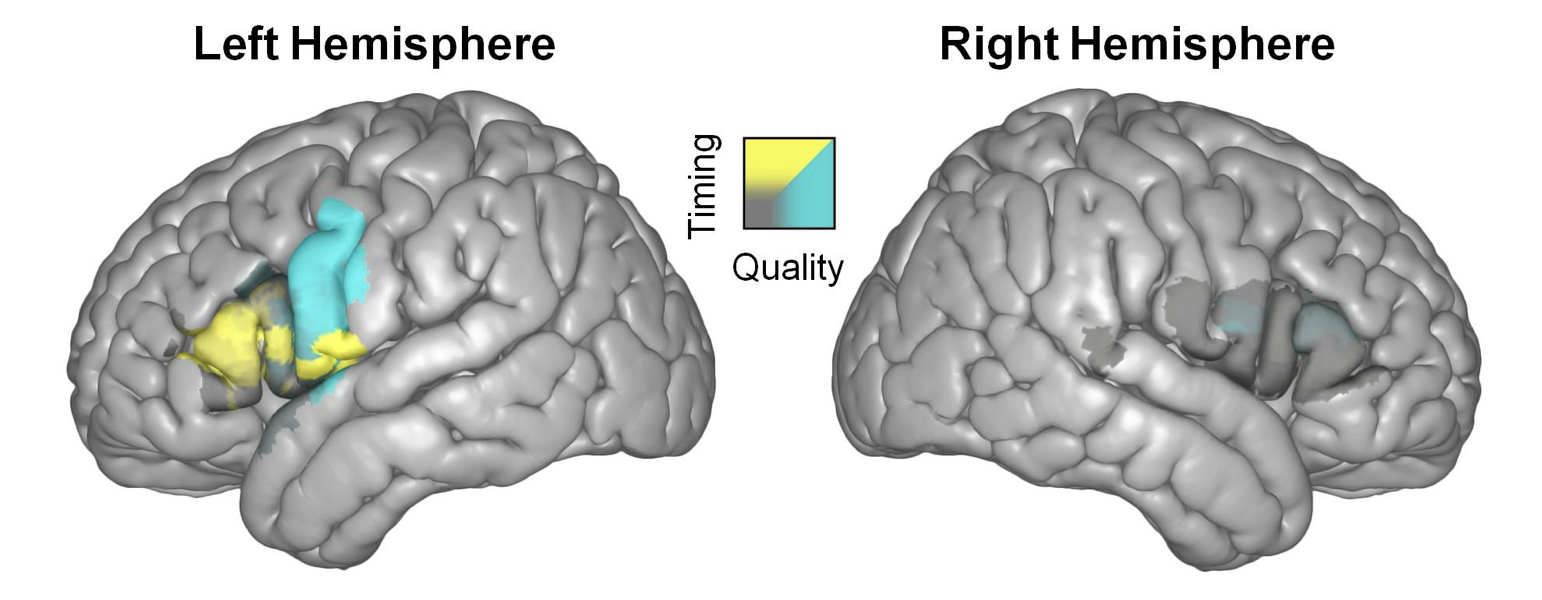
\includegraphics[width=0.85\textwidth]{images/neuro}    		
    	\end{center}
    	\textit{A functional map showing cooling in both hemispheres.} \cite{longResearchLongLab}
    	
    	Dr. Long's group has made numerous contributions to the fields of vocalization and speech analysis, including work with understanding the role of the inhibitory cells in the brain, which could help researchers develop ways to manipulate such networks.
    \end{block}
\end{column}
\begin{column}{0.55\textwidth - 1cm}


%%%%%%%%%%%%%%%%%%%%%%%%%%%%%%%%%%%%%%%%%%%%%%%%%%%%%
%                 BLOCK: ABSTRACT                   %
%%%%%%%%%%%%%%%%%%%%%%%%%%%%%%%%%%%%%%%%%%%%%%%%%%%%%
    \begin{block}{Talk Abstract}
    	Vocal communication is central to our everyday lives, facilitating social exchange. Despite significant recent discoveries, the neural mechanisms underlying coordinated vocal exchanges remain poorly understood. We examine the brain processes involved in interactive vocal behaviors, focusing on forebrain circuitry in the songbird and the rodent, and we relate these to emerging human studies that employ a range of methods to manipulate and monitor cortical areas relevant for speech.
    \end{block}


%%%%%%%%%%%%%%%%%%%%%%%%%%%%%%%%%%%%%%%%%%%%%%%%%%%%%
%                BLOCK: BACKGROUND                  %
%%%%%%%%%%%%%%%%%%%%%%%%%%%%%%%%%%%%%%%%%%%%%%%%%%%%%
    \begin{block}{Brief Background}
    	Complex behaviors, like interaction with the outside world, are made possible by the ability of the brain to carry out sequences of neural states; motor sequencing, navigation, movement planning and certain cognitive tasks. Even though speech and communicative gestures are central to everyday life, the neural underpinnings of these learned motor sequences are poorly understood. The Long Lab seeks to identify the relevant processing centers involved in producing specific motor sequences through careful circuit manipulation and to investigate their functional properties during natural behavior. To accomplish this, they focus on three distinct types of behaviors notable for their roles in enabling vocal communication.  
    	\cite{longLocalAxonalConduction2020} 
        \begin{center}
		   	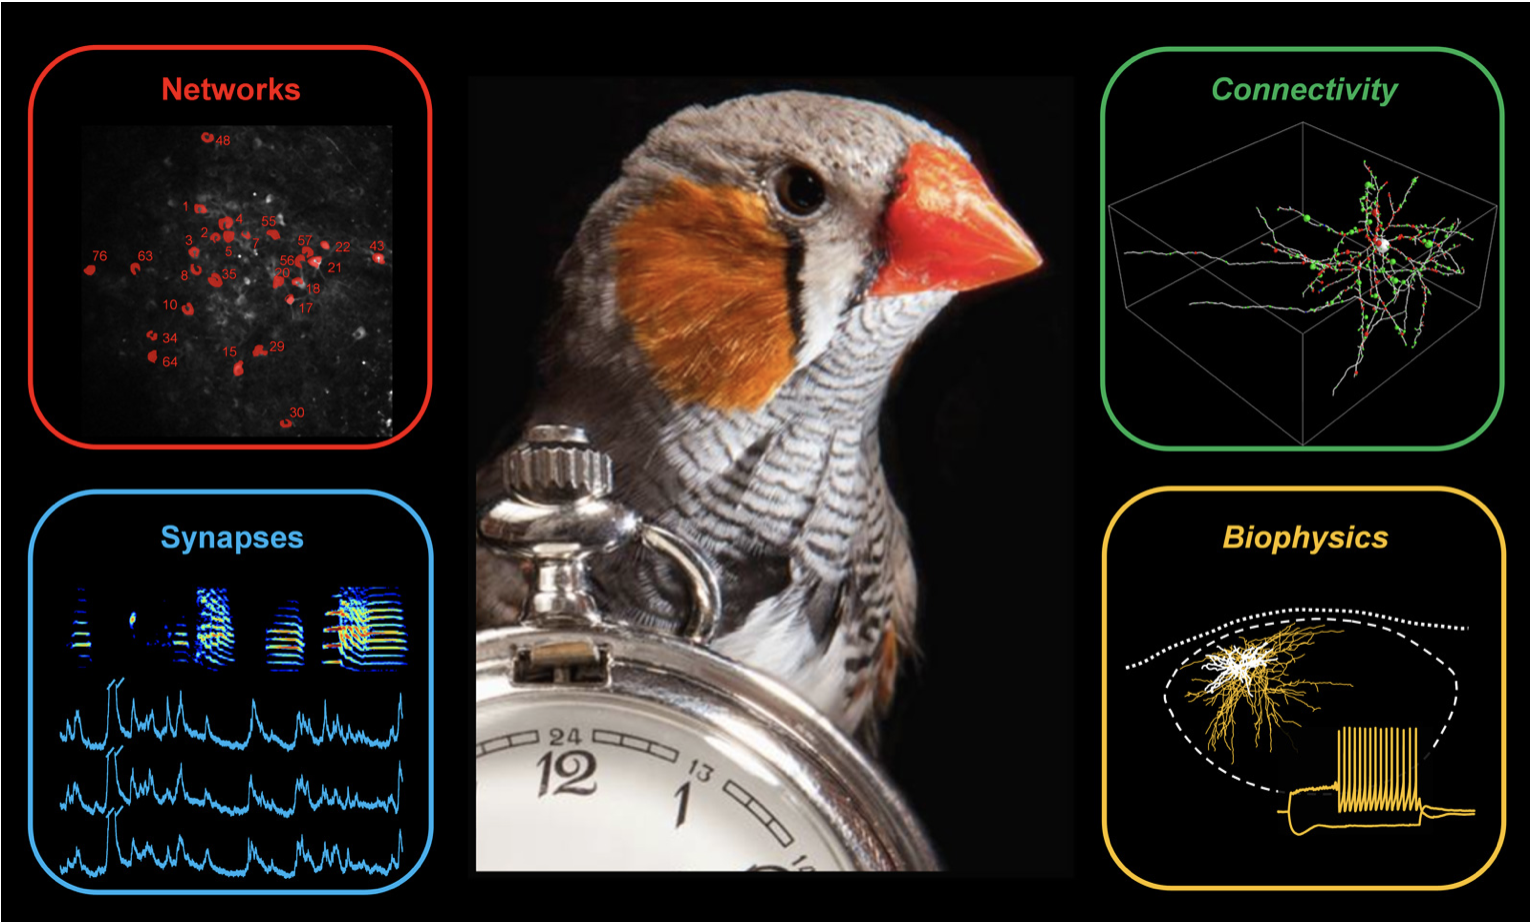
\includegraphics[width=0.95\textwidth]{images/bird}    		
    	\end{center}
		The lab studies song production in the zebra finch (Taenjopygia guttata) songbird to uncover the circuit principles that enable sequence generation during a well-characterized learned behavior, countersinging in a neotropical rodent (Scotinomys teguina), and activation of different regions involved in human speech. 
		\cite{longMorphologicalCharacterizationHVC2018} 
    \end{block}


%%%%%%%%%%%%%%%%%%%%%%%%%%%%%%%%%%%%%%%%%%%%%%%%%%%%%
%                 BLOCK: REFERENCES                 %
%%%%%%%%%%%%%%%%%%%%%%%%%%%%%%%%%%%%%%%%%%%%%%%%%%%%%
    \begin{block}{References}
        \bibliographystyle{aipnum4-1}
%        \bibliographystyle{iopart-num}
		\bibliography{../references}
    \end{block}

\end{column}
\end{columns}


%%%%%%%%%%%%%%%%%%%%%%%%%%%%%%%%%%%%%%%%%%%%%%%%%%%%%
%                    FOOTER TEXT                    %
%%%%%%%%%%%%%%%%%%%%%%%%%%%%%%%%%%%%%%%%%%%%%%%%%%%%%
\begin{textblock}{0.5}(0.18, 0.94)
    \color{white}
    \sffamily
    \textbf{Eberly College of Science}
    \\
    Department of Physics
\end{textblock}


%%%%%%%%%%%%%%%%%%%%%%%%%%%%%%%%%%%%%%%%%%%%%%%%%%%%%
%                   END TEMPLATE                    %
%%%%%%%%%%%%%%%%%%%%%%%%%%%%%%%%%%%%%%%%%%%%%%%%%%%%%
\end{frame}
\end{document}
